
%% bare_conf.tex
%% V1.3
%% 2007/01/11
%% by Michael Shell
%% See:
%% http://www.michaelshell.org/
%% for current contact information.
%%
%% This is a skeleton file demonstrating the use of IEEEtran.cls
%% (requires IEEEtran.cls version 1.7 or later) with an IEEE conference paper.
%%
%% Support sites:
%% http://www.michaelshell.org/tex/ieeetran/
%% http://www.ctan.org/tex-archive/macros/latex/contrib/IEEEtran/
%% and
%% http://www.ieee.org/

%%*************************************************************************
%% Legal Notice:
%% This code is offered as-is without any warranty either expressed or
%% implied; without even the implied warranty of MERCHANTABILITY or
%% FITNESS FOR A PARTICULAR PURPOSE! 
%% User assumes all risk.
%% In no event shall IEEE or any contributor to this code be liable for
%% any damages or losses, including, but not limited to, incidental,
%% consequential, or any other damages, resulting from the use or misuse
%% of any information contained here.
%%
%% All comments are the opinions of their respective authors and are not
%% necessarily endorsed by the IEEE.
%%
%% This work is distributed under the LaTeX Project Public License (LPPL)
%% ( http://www.latex-project.org/ ) version 1.3, and may be freely used,
%% distributed and modified. A copy of the LPPL, version 1.3, is included
%% in the base LaTeX documentation of all distributions of LaTeX released
%% 2003/12/01 or later.
%% Retain all contribution notices and credits.
%% ** Modified files should be clearly indicated as such, including  **
%% ** renaming them and changing author support contact information. **
%%
%% File list of work: IEEEtran.cls, IEEEtran_HOWTO.pdf, bare_adv.tex,
%%                    bare_conf.tex, bare_jrnl.tex, bare_jrnl_compsoc.tex
%%*************************************************************************

% *** Authors should verify (and, if needed, correct) their LaTeX system  ***
% *** with the testflow diagnostic prior to trusting their LaTeX platform ***
% *** with production work. IEEE's font choices can trigger bugs that do  ***
% *** not appear when using other class files.                            ***
% The testflow support page is at:
% http://www.michaelshell.org/tex/testflow/



% Note that the a4paper option is mainly intended so that authors in
% countries using A4 can easily print to A4 and see how their papers will
% look in print - the typesetting of the document will not typically be
% affected with changes in paper size (but the bottom and side margins will).
% Use the testflow package mentioned above to verify correct handling of
% both paper sizes by the user's LaTeX system.
%
% Also note that the "draftcls" or "draftclsnofoot", not "draft", option
% should be used if it is desired that the figures are to be displayed in
% draft mode.
%
\documentclass[conference]{IEEEtran}
% Add the compsoc option for Computer Society conferences.
%
% If IEEEtran.cls has not been installed into the LaTeX system files,
% manually specify the path to it like:
% \documentclass[conference]{../sty/IEEEtran}





% Some very useful LaTeX packages include:
% (uncomment the ones you want to load)


% *** MISC UTILITY PACKAGES ***
%
%\usepackage{ifpdf}
% Heiko Oberdiek's ifpdf.sty is very useful if you need conditional
% compilation based on whether the output is pdf or dvi.
% usage:
% \ifpdf
%   % pdf code
% \else
%   % dvi code
% \fi
% The latest version of ifpdf.sty can be obtained from:
% http://www.ctan.org/tex-archive/macros/latex/contrib/oberdiek/
% Also, note that IEEEtran.cls V1.7 and later provides a builtin
% \ifCLASSINFOpdf conditional that works the same way.
% When switching from latex to pdflatex and vice-versa, the compiler may
% have to be run twice to clear warning/error messages.






% *** CITATION PACKAGES ***
%
\usepackage{cite}
% cite.sty was written by Donald Arseneau
% V1.6 and later of IEEEtran pre-defines the format of the cite.sty package
% \cite{} output to follow that of IEEE. Loading the cite package will
% result in citation numbers being automatically sorted and properly
% "compressed/ranged". e.g., [1], [9], [2], [7], [5], [6] without using
% cite.sty will become [1], [2], [5]--[7], [9] using cite.sty. cite.sty's
% \cite will automatically add leading space, if needed. Use cite.sty's
% noadjust option (cite.sty V3.8 and later) if you want to turn this off.
% cite.sty is already installed on most LaTeX systems. Be sure and use
% version 4.0 (2003-05-27) and later if using hyperref.sty. cite.sty does
% not currently provide for hyperlinked citations.
% The latest version can be obtained at:
% http://www.ctan.org/tex-archive/macros/latex/contrib/cite/
% The documentation is contained in the cite.sty file itself.






% *** GRAPHICS RELATED PACKAGES ***
%
\ifCLASSINFOpdf
  % \usepackage[pdftex]{graphicx}
  % declare the path(s) where your graphic files are
  % \graphicspath{{../pdf/}{../jpeg/}}
  % and their extensions so you won't have to specify these with
  % every instance of \includegraphics
  % \DeclareGraphicsExtensions{.pdf,.jpeg,.png}
\else
  % or other class option (dvipsone, dvipdf, if not using dvips). graphicx
  % will default to the driver specified in the system graphics.cfg if no
  % driver is specified.
  % \usepackage[dvips]{graphicx}
  % declare the path(s) where your graphic files are
  % \graphicspath{{../eps/}}
  % and their extensions so you won't have to specify these with
  % every instance of \includegraphics
  % \DeclareGraphicsExtensions{.eps}
\fi
% graphicx was written by David Carlisle and Sebastian Rahtz. It is
% required if you want graphics, photos, etc. graphicx.sty is already
% installed on most LaTeX systems. The latest version and documentation can
% be obtained at: 
% http://www.ctan.org/tex-archive/macros/latex/required/graphics/
% Another good source of documentation is "Using Imported Graphics in
% LaTeX2e" by Keith Reckdahl which can be found as epslatex.ps or
% epslatex.pdf at: http://www.ctan.org/tex-archive/info/
%
% latex, and pdflatex in dvi mode, support graphics in encapsulated
% postscript (.eps) format. pdflatex in pdf mode supports graphics
% in .pdf, .jpeg, .png and .mps (metapost) formats. Users should ensure
% that all non-photo figures use a vector format (.eps, .pdf, .mps) and
% not a bitmapped formats (.jpeg, .png). IEEE frowns on bitmapped formats
% which can result in "jaggedy"/blurry rendering of lines and letters as
% well as large increases in file sizes.
%
% You can find documentation about the pdfTeX application at:
% http://www.tug.org/applications/pdftex





% *** MATH PACKAGES ***
%
%\usepackage[cmex10]{amsmath}
% A popular package from the American Mathematical Society that provides
% many useful and powerful commands for dealing with mathematics. If using
% it, be sure to load this package with the cmex10 option to ensure that
% only type 1 fonts will utilized at all point sizes. Without this option,
% it is possible that some math symbols, particularly those within
% footnotes, will be rendered in bitmap form which will result in a
% document that can not be IEEE Xplore compliant!
%
% Also, note that the amsmath package sets \interdisplaylinepenalty to 10000
% thus preventing page breaks from occurring within multiline equations. Use:
%\interdisplaylinepenalty=2500
% after loading amsmath to restore such page breaks as IEEEtran.cls normally
% does. amsmath.sty is already installed on most LaTeX systems. The latest
% version and documentation can be obtained at:
% http://www.ctan.org/tex-archive/macros/latex/required/amslatex/math/





% *** SPECIALIZED LIST PACKAGES ***
%
%\usepackage{algorithmic}
% algorithmic.sty was written by Peter Williams and Rogerio Brito.
% This package provides an algorithmic environment fo describing algorithms.
% You can use the algorithmic environment in-text or within a figure
% environment to provide for a floating algorithm. Do NOT use the algorithm
% floating environment provided by algorithm.sty (by the same authors) or
% algorithm2e.sty (by Christophe Fiorio) as IEEE does not use dedicated
% algorithm float types and packages that provide these will not provide
% correct IEEE style captions. The latest version and documentation of
% algorithmic.sty can be obtained at:
% http://www.ctan.org/tex-archive/macros/latex/contrib/algorithms/
% There is also a support site at:
% http://algorithms.berlios.de/index.html
% Also of interest may be the (relatively newer and more customizable)
% algorithmicx.sty package by Szasz Janos:
% http://www.ctan.org/tex-archive/macros/latex/contrib/algorithmicx/




% *** ALIGNMENT PACKAGES ***
%
%\usepackage{array}
% Frank Mittelbach's and David Carlisle's array.sty patches and improves
% the standard LaTeX2e array and tabular environments to provide better
% appearance and additional user controls. As the default LaTeX2e table
% generation code is lacking to the point of almost being broken with
% respect to the quality of the end results, all users are strongly
% advised to use an enhanced (at the very least that provided by array.sty)
% set of table tools. array.sty is already installed on most systems. The
% latest version and documentation can be obtained at:
% http://www.ctan.org/tex-archive/macros/latex/required/tools/


%\usepackage{mdwmath}
%\usepackage{mdwtab}
% Also highly recommended is Mark Wooding's extremely powerful MDW tools,
% especially mdwmath.sty and mdwtab.sty which are used to format equations
% and tables, respectively. The MDWtools set is already installed on most
% LaTeX systems. The lastest version and documentation is available at:
% http://www.ctan.org/tex-archive/macros/latex/contrib/mdwtools/


% IEEEtran contains the IEEEeqnarray family of commands that can be used to
% generate multiline equations as well as matrices, tables, etc., of high
% quality.


%\usepackage{eqparbox}
% Also of notable interest is Scott Pakin's eqparbox package for creating
% (automatically sized) equal width boxes - aka "natural width parboxes".
% Available at:
% http://www.ctan.org/tex-archive/macros/latex/contrib/eqparbox/





% *** SUBFIGURE PACKAGES ***
%\usepackage[tight,footnotesize]{subfigure}
% subfigure.sty was written by Steven Douglas Cochran. This package makes it
% easy to put subfigures in your figures. e.g., "Figure 1a and 1b". For IEEE
% work, it is a good idea to load it with the tight package option to reduce
% the amount of white space around the subfigures. subfigure.sty is already
% installed on most LaTeX systems. The latest version and documentation can
% be obtained at:
% http://www.ctan.org/tex-archive/obsolete/macros/latex/contrib/subfigure/
% subfigure.sty has been superceeded by subfig.sty.



%\usepackage[caption=false]{caption}
%\usepackage[font=footnotesize]{subfig}
% subfig.sty, also written by Steven Douglas Cochran, is the modern
% replacement for subfigure.sty. However, subfig.sty requires and
% automatically loads Axel Sommerfeldt's caption.sty which will override
% IEEEtran.cls handling of captions and this will result in nonIEEE style
% figure/table captions. To prevent this problem, be sure and preload
% caption.sty with its "caption=false" package option. This is will preserve
% IEEEtran.cls handing of captions. Version 1.3 (2005/06/28) and later 
% (recommended due to many improvements over 1.2) of subfig.sty supports
% the caption=false option directly:
\usepackage[caption=false,font=footnotesize]{subfig}
%
% The latest version and documentation can be obtained at:
% http://www.ctan.org/tex-archive/macros/latex/contrib/subfig/
% The latest version and documentation of caption.sty can be obtained at:
% http://www.ctan.org/tex-archive/macros/latex/contrib/caption/




% *** FLOAT PACKAGES ***
%
%\usepackage{fixltx2e}
% fixltx2e, the successor to the earlier fix2col.sty, was written by
% Frank Mittelbach and David Carlisle. This package corrects a few problems
% in the LaTeX2e kernel, the most notable of which is that in current
% LaTeX2e releases, the ordering of single and double column floats is not
% guaranteed to be preserved. Thus, an unpatched LaTeX2e can allow a
% single column figure to be placed prior to an earlier double column
% figure. The latest version and documentation can be found at:
% http://www.ctan.org/tex-archive/macros/latex/base/



%\usepackage{stfloats}
% stfloats.sty was written by Sigitas Tolusis. This package gives LaTeX2e
% the ability to do double column floats at the bottom of the page as well
% as the top. (e.g., "\begin{figure*}[!b]" is not normally possible in
% LaTeX2e). It also provides a command:
%\fnbelowfloat
% to enable the placement of footnotes below bottom floats (the standard
% LaTeX2e kernel puts them above bottom floats). This is an invasive package
% which rewrites many portions of the LaTeX2e float routines. It may not work
% with other packages that modify the LaTeX2e float routines. The latest
% version and documentation can be obtained at:
% http://www.ctan.org/tex-archive/macros/latex/contrib/sttools/
% Documentation is contained in the stfloats.sty comments as well as in the
% presfull.pdf file. Do not use the stfloats baselinefloat ability as IEEE
% does not allow \baselineskip to stretch. Authors submitting work to the
% IEEE should note that IEEE rarely uses double column equations and
% that authors should try to avoid such use. Do not be tempted to use the
% cuted.sty or midfloat.sty packages (also by Sigitas Tolusis) as IEEE does
% not format its papers in such ways.





% *** PDF, URL AND HYPERLINK PACKAGES ***
%
\usepackage{url}
% url.sty was written by Donald Arseneau. It provides better support for
% handling and breaking URLs. url.sty is already installed on most LaTeX
% systems. The latest version can be obtained at:
% http://www.ctan.org/tex-archive/macros/latex/contrib/misc/
% Read the url.sty source comments for usage information. Basically,
% \url{my_url_here}.





% *** Do not adjust lengths that control margins, column widths, etc. ***
% *** Do not use packages that alter fonts (such as pslatex).         ***
% There should be no need to do such things with IEEEtran.cls V1.6 and later.
% (Unless specifically asked to do so by the journal or conference you plan
% to submit to, of course. )


% correct bad hyphenation here
\hyphenation{op-tical net-works semi-conduc-tor}

%%% My packages
\usepackage{amsmath,epsfig}
\usepackage{amsfonts}

%%% My commands
\newcommand{\mat}[1]{\mathbf{#1}}
\renewcommand{\vec}[1]{\mathbf{#1}}
\newcommand{\degree}{\ensuremath{^\circ}}


\begin{document}
%
% paper title
% can use linebreaks \\ within to get better formatting as desired
\title{Implementing Capon Adaptive Beamforming on the GPU for Real Time Cardiac Ultrasound Imaging}


% author names and affiliations
% use a multiple column layout for up to three different
% affiliations
\author{
\IEEEauthorblockN{
Jon Petter \AA{}sen\IEEEauthorrefmark{1},
Jo Inge Buskenes\IEEEauthorrefmark{2},
Carl-Inge C. Nilsen\IEEEauthorrefmark{2},
Andreas Austeng\IEEEauthorrefmark{2},
Sverre Holm\IEEEauthorrefmark{1}\IEEEauthorrefmark{2}
}
\IEEEauthorblockA{
\IEEEauthorrefmark{1} Mi Lab, Norwegian University of Science and Technology, Trondheim, Norway,\\
\IEEEauthorrefmark{2} Department of Informatics, University of Oslo, Oslo, Norway
}
}

% conference papers do not typically use \thanks and this command
% is locked out in conference mode. If really needed, such as for
% the acknowledgment of grants, issue a \IEEEoverridecommandlockouts
% after \documentclass

% for over three affiliations, or if they all won't fit within the width
% of the page, use this alternative format:
% 
%\author{\IEEEauthorblockN{Michael Shell\IEEEauthorrefmark{1},
%Homer Simpson\IEEEauthorrefmark{2},
%James Kirk\IEEEauthorrefmark{3}, 
%Montgomery Scott\IEEEauthorrefmark{3} and
%Eldon Tyrell\IEEEauthorrefmark{4}}
%\IEEEauthorblockA{\IEEEauthorrefmark{1}School of Electrical and Computer Engineering\\
%Georgia Institute of Technology,
%Atlanta, Georgia 30332--0250\\ Email: see http://www.michaelshell.org/contact.html}
%\IEEEauthorblockA{\IEEEauthorrefmark{2}Twentieth Century Fox, Springfield, USA\\
%Email: homer@thesimpsons.com}
%\IEEEauthorblockA{\IEEEauthorrefmark{3}Starfleet Academy, San Francisco, California 96678-2391\\
%Telephone: (800) 555--1212, Fax: (888) 555--1212}
%\IEEEauthorblockA{\IEEEauthorrefmark{4}Tyrell Inc., 123 Replicant Street, Los Angeles, California 90210--4321}}




% use for special paper notices
%\IEEEspecialpapernotice{(Invited Paper)}




% make the title area
\maketitle


\begin{abstract}
\boldmath
Recent results \cite{Synnevag2007, Austeng2008, Vignon2008, Viola, Mehdizadeh2012} suggest that the Capon beamformer can provide increased lateral resolution when applied in medical ultrasound imaging. In this paper, the high computational complexity of the Capon beamformer is targeted with the use of Graphics Processing Units (GPUs). We also present in-vivo results with Capon beamforming applied on a full cardiac cycle in addition to simulations. With GPUs we are able to process a $70\degree$ sector cardiac image from a 64 element phased array at interactive frame rates using both spatial and temporal smoothing.

For a typical cardiac ultrasound image of $80\times400$ pixels ($70\degree$ sector, 15cm range) acquired using a 2.5MHz, M=64 element phased array, we obtain 10 fps (subarray length L=M/2, temporal smoothing over 3 samples). If we do a 2-element pre-beamforming to get the channel count down to 32, the frame rate increases to 44 fps. For a 32 element phased array we need less beams to cover the sector ($40\times400$ pixels), hence with the same parameters the frame rate increases to 87 fps. After optimization the bottleneck of the Capon algorithm is to find the inverse covariance matrix for all pixels. This is an $O(L^3)$ operation, and when L is larger than 16 (M = 64), real time performance is not possible for cardiac imaging with current high-end hardware. The target GPU has been Nvidia’s Quadro 6000, capable of 1 Tflops.

\end{abstract}
% IEEEtran.cls defaults to using nonbold math in the Abstract.
% This preserves the distinction between vectors and scalars. However,
% if the conference you are submitting to favors bold math in the abstract,
% then you can use LaTeX's standard command \boldmath at the very start
% of the abstract to achieve this. Many IEEE journals/conferences frown on
% math in the abstract anyway.

% no keywords




% For peer review papers, you can put extra information on the cover
% page as needed:
% \ifCLASSOPTIONpeerreview
% \begin{center} \bfseries EDICS Category: 3-BBND \end{center}
% \fi
%
% For peerreview papers, this IEEEtran command inserts a page break and
% creates the second title. It will be ignored for other modes.
\IEEEpeerreviewmaketitle



\section{Introduction}
Capon adaptive beamforming \cite{Capon1969} applied to medical ultrasound imaging has recently shown promising results in several studies \cite{Synnevag2007, Austeng2008, Vignon2008, Viola, Mehdizadeh2012}. For instance, some interesting trade-offs in addition to just improved resolution were introduced, like maintaining image resolution in combination with higher framerates, smaller probes, or deeper penetration \cite{Synnevag2009}. Despite these benefits, widespread use has been limited by the immense computational complexity associated with the method \cite{So2011}.  In this paper we introduce the first implementation of the Capon beamformer exhibiting real-time performance when applied in a typical cardiac ultrasound imaging setting. To accomplish this task we make use of the massive, and easily accessed, parallel processing power found in modern Graphics Processing Units (GPUs). 

Previous work on implementing a parallel Capon beamformer has mainly been focused around radar and passive sonar systems using custom made systolic array processors \cite{McWhirter1989, Sinha2002}. For medical ultrasound, Chen et al. \cite{Chen2011a, Chen2011} have implemented a Capon beamformer on the GPU that produced real apodization weights based on real data. Under this constraint the Capon beamformer is not allowed to micro steer the main lobe, and therefore its full potential is not reached. Micro steering of the main lobe is an important property of the Capon beamformer in order for it to improve edge definitions and contrast throughout an ultrasound image. Another aspect of using complex data is that even though the number of aritmetic operations per sample is increased we can now sample at the system bandwidth, keeping the number of samples for a full cardiac imaging sector at a minimum. All results in this paper are reported with the use of baseband data.

%In the next section we present background information about the Capon beamformer and the GPU computing model. In Section \ref{sec:meth} we go in detail about the parallel implementation of the Capon beamformer, before in Section \ref{sec:bs} we introduce the method applied when the problem size increases. Benchmark results and resulting images are presented in Section \ref{sec:res}, and finally we discuss the results in Section \ref{sec:dis}, and draw conclusions in Section \ref{sec:con}. 


\section{Background}
\subsection{Capon Adaptive Beamforming}
The conventional form of array beamforming is delay-and-sum (DAS). Here, the signal $x_m[n]$ recorded at element number $m \in [0,M-1]$ at time $n$ is delayed to broadside with an appropriate delay $\Delta_m[n]$. The beamformer output, $z[n]$, is then the sum of all $M$ channels weighted with a per-element factor $w_m$,
\begin{align}
z[n] = \sum_{m = 0}^{M-1}w_m^*x_m[n - \Delta_m[n]] = \vec{w}^H\vec{x}^{\Delta}[n]. \label{eq:z}
\end{align}
In conventional beamforming, the weighting $\vec{w}$ is usually real, and is applied to trade resolution for a better signal-to-noise ratio (SNR).

As shown in Figure \ref{fig:mvbf}, the basic idea of an adaptive beamformer is to form a weight vector based on the data at hand.  For Capon adaptive beamforming the weights are found that minimize the beamformer output power while maintaining unit gain at broadside. The result is that interference impinging from other directions than the point of focus is suppressed \cite{Synnevag2007}.
%\textbf{(Vi skal implementer dette. vis bare vektene. Dropp ligning 2, siter, bruk R-hat med en gang. Få med den endelige feilen )}

%Formally stated, the adaptive weights are found by solving the following minimization problem:
%\begin{align}
%&\min_{\vec{w}} E\{|z[n]|^2\} = \min_{\vec{w}}\vec{w}^H\mat{R}\vec{w}\label{eq:minz}\\
%&\text{subjected to } \vec{w}^H\vec{a} = 1,\label{eq:constraint}
%\end{align}
%where $\mat{R} = E\{\vec{x}[n]\vec{x}[n]^H\}$ is the spatial covariance matrix, and $\vec{a} = \left[ \begin{array}{cccc} e^{-jk_{\tilde{x}}\tilde{x}_0}& e^{-jk_{\tilde{x}}\tilde{x}_1}& ...& e^{-jk_{\tilde{x}}\tilde{x}_{M-1}}\end{array}\right] ^T$ is a far-field steering vector towards angle $\theta = \arcsin(\frac{\lambda k_{\tilde{x}}}{2\pi})$.
%The constraint in (\ref{eq:constraint}) is there to avoid the trivial solution $\vec{w} = 0$, and a distorted respons in the direction of $\vec{a}$. 
%The solution to the minimization problem in (\ref{eq:minz}) and (\ref{eq:constraint}) is

\begin{figure}
\centerline{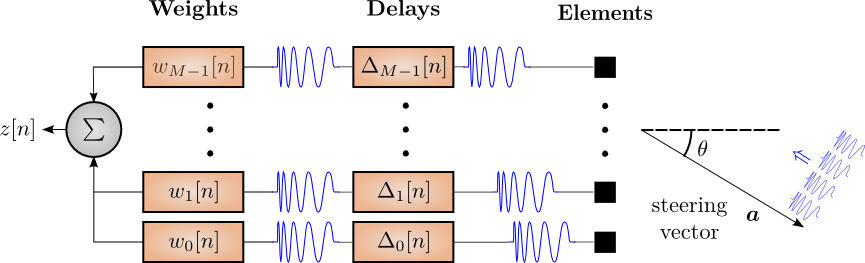
\includegraphics[width=3in]{gfx/beamforming_mv_lowres.png}}
\caption{Adaptive beamforming. Impinging signal is demodulated, and aligned in phase by applying steering and focusing delays $\Delta_m[n]$. Adaptive weights, $\vec{w}[n]$, are then calculated based on in-phase data, and finally the output is formed by a weighted coherent sum.}
\label{fig:mvbf}
\end{figure}

To calculate the Capon beamformer output we need three equations. First the sample covariance matrix has to be calculated,
\begin{align}
\mat{\breve{R}}[n] = \frac{1}{N_LN_K}\sum_{n'=n-K}^{n+K} \sum_{l=0}^{N_L-1} \vec{x}_l^{\Delta}[n']\vec{x}_l^{\Delta}[n']^H,\label{eq:R}
\end{align}
where  $N_K = 2K + 1$ is the number of samples included in time, $N_L = M-L+1$ is the number of subarrays, and $\vec{x}_l^{\Delta}$ is the $l^\text{th}$ subarray $[x_l^{\Delta}[n], \dotso, x_{l+L-1}^{\Delta}[n]]$. Note that the dimension of the covariance matrix is $L \times L$. The covariance matrix is usually loaded with a diagonal factor $\epsilon$ to ensure numerical stability, 
\begin{align}\label{eq:diag}
\mat{\hat{R}} = \mat{\breve{R}} + \epsilon\mat{I}.
\end{align}
A weighting proportional to the output power is often used to reduce the need of parameter adjustments, and the trace of $\mat{\breve{R}}$, 
\begin{align}\label{eq:diag_adapt}
\epsilon &= d \times tr\{\mat{\breve{R}}\}, \\
d &= 1/L
\end{align}
has been applied in much of the resent literature on Capon beamforming for medical ultrasound imaging \cite{Synnevag2007, Mehdizadeh2012}.

Second, we calculate the Capon weight vector as
\begin{align}\label{eq:w}
\vec{w}[n] = \frac{\mat{\hat{R}}[n]^{-1}\vec{a}}{\vec{a}^H\mat{\hat{R}}[n]^{-1}\vec{a}} = \frac{\vec{b}}{\vec{a}^H\vec{b}},
\end{align}
where $\vec{a} = [1_0, 1_1, ..., 1_{L-1}]^T = \vec{1}_L$ when $\vec{x}$ is pre-delayed. 

And last, the beamformer output is calculated by combining all $N_L$ subarrays weighted with the same set of adaptive weights,
\begin{align}
z[n] &= \frac{1}{N_L}\vec{w}[n]^H \sum_{l=0}^{N_L-1} \vec{x}_l^{\Delta}[n]. \label{eq:z_mv}
\end{align}

%The Capon weight vector is given by the following expression:
%\begin{align}\label{eq:w}
%\vec{w}[n] = \frac{\mat{\hat{R}}[n]^{-1}\vec{a}}{\vec{a}^H\mat{\hat{R}}[n]^{-1}\vec{a}} = \frac{\vec{b}}{\vec{a}^H\vec{b}},
%\end{align}
%where $\vec{a} = [1_0, 1_1, ..., 1_{M-1}]^T = \vec{1}_M$ when $\vec{x}$ is pre-delayed, $\mat{\hat{R}}$ is the sample covariance matrix calculated from %the data vector $\vec{x}^\Delta[n]$, and $\vec{b} = \mat{\hat{R}}[n]^{-1}\vec{a}$. 

%In order to get a well-conditioned $\mat{\hat{R}}$, avoid signal cancellation, and to get DAS-like speckle, $\mat{\hat{R}}$ has to be averaged over $L\le M/2$ long subarrays and $N_K \sim T_p/T_s$ time samples \cite{Synnevag2007, Synnevag2007a}. Where, $T_p$ is the pulse length in seconds and $T_s$ is the sampling period. We therefore calculate
%\begin{align}
%\mat{\breve{R}}[n] = \frac{1}{N_LN_K}\sum_{n'=n-K}^{n+K} \sum_{l=0}^{N_L-1} \vec{x}_l^{\Delta}[n']\vec{x}_l^{\Delta}[n']^H,\label{eq:R}
%\end{align}
%where  $N_K = 2K + 1$ is the number of samples included in time, $N_L = M-L+1$ is the number of subarrays, and $\vec{x}_l^{\Delta}$ is the $l^\text{th}$ subarray $[x_l^{\Delta}[n], \dotso, x_{l+L-1}^{\Delta}[n]]$. The dimension of the covariance matrix after this smoothing is $L \times L$. Hence, the size of $\vec{w}[n]$ and $\vec{a}$ in (\ref{eq:w}) has to be $L \times 1$ when the covariance matrix in (\ref{eq:R}) is used.
%Finally, the covariance matrix is loaded with a diagonal factor $\epsilon$ to ensure numerical stability, 
%\begin{align}\label{eq:diag}
%\mat{\hat{R}} = \mat{\breve{R}} + \epsilon\mat{I}.
%\end{align}
%A weighting proportional to the output power is often used to reduce the need of parameter adjustments, and the trace of $\mat{\breve{R}}$, 
%\begin{align}\label{eq:diag_adapt}
%\epsilon &= d \times tr\{\mat{\breve{R}}\}, \\
%d &= 1/L
%\end{align}
%has been applied in much of the resent literature on Capon beamforming for medical ultrasound imaging \cite{Synnevag2007, Wang2009, Mehdizadeh2012}.

%The beamformer output is in the end calculated by combining all $N_L$ subarrays weighted with the same set of adaptive weights,
%\begin{align}
%z[n] &= \frac{1}{N_L}\vec{w}[n]^H \sum_{l=0}^{N_L-1} \vec{x}_l^{\Delta}[n]. \label{eq:z_mv}
%\end{align}

\subsection{GPU Compute Model}
CUDA by Nvidia has been our choice of GPU developer environment \cite{Nvidia2011}. The CUDA compute model is based on execution of a kernel function across a grid of compute threads, where the kernel function describes the work to be done by each thread. As depicted in Figure \ref{fig:gpulayout}, each position in the grid holds a block of threads, with maximal size of 1024 threads, that can be synchronized with little cost if needed. 
%Each block is further divided into groups of 32 threads, known as a warp. The maximum number of threads inside a block is restricted to 512, hence 16 warps. 
From a CUDA perspective the GPU consists of one or more stream multi processors (SMs), where each SM is capable of 32 or more, depending on the architecture, concurrent multiplications and/or additions. A group of blocks is scheduled to each SM until all blocks have been processed. 

A SM has available a limited amount of near-core memory and registers. Each thread therefore has to be as light on memory as possible and has to perform enough instructions per used byte in order to hide memory latency. Global reads and writes on the GPU, in addition to CPU-GPU transfers, have high penalty, and should be minimized as much as possible. All of these constraints combined pose a real challenge as the target problem has to map on to the parallel framework both on a grid, block and memory consumption level in order to benefits from parallel acceleration. In the next section, we will describe how this mapping can be done for Capon beamforming of cardiac ultrasound data.    

\begin{figure}
\centerline{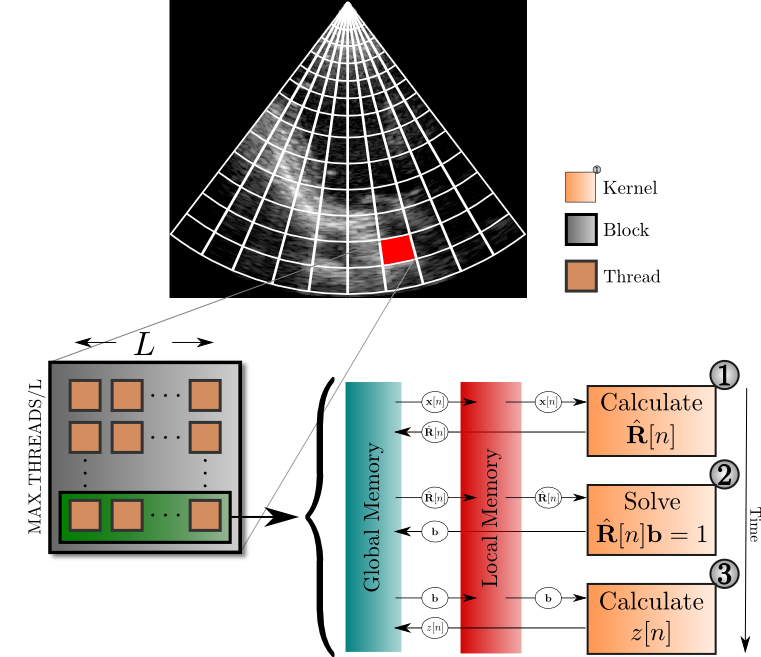
\includegraphics[width=3in]{gfx/gpu_layout_vertical_lr.png}}
\caption{Calculation of Capon adaptive weights mapped to GPU architecture. A recorded echo across the array for a given range and angle (selected cell) is assigned to a group of $L$ threads that can run independently of all other groups. Note that several samples can be processed per block of threads if $L$ is small. The task of these $L$ threads is to calculate the Capon beamformer output in the three depicted steps.}
\label{fig:gpulayout}
\end{figure}


\section{Parallel Capon}\label{sec:meth}
If we analyze the beamformer in (\ref{eq:z_mv}) in combination with (\ref{eq:w}) and (\ref{eq:R}), we see that each calculation of a set of Capon weights is independent across the outputs $z[n]$. As shown in Figure \ref{fig:gpulayout}, a first level of granularity is therefore to divide the image into a grid, where the output in each cell can be calculated independently of all others. Further, based on memory dependencies and to hold memory consumption per thread at a minimum, one should recognise that a group of threads should process one output in the final image. Continuing with the calculation of one weight vector, the algorithm can be broken down into three main steps that, to some extent, can be further divided into a small set of parallel processes. That is, for each data vector $\vec{x}^\Delta$ in the image:
\begin{align*}
%\begin{array}{l}
\text{1) } &\text{Calculate the sample covariance matrix } \mat{\hat{R}} \text{ as in } \text{(\ref{eq:diag})}\\
\text{2) } &\text{Solve the linear system of equations } \vec{b} =\mat{\hat{R}}^{-1}\vec{1}_L\\
\text{3) } &\text{Calculate } \vec{w} = \vec{b}/\vec{1}_{L}^H\vec{b} \text{ and the amplitude as in (\ref{eq:z_mv})}
%\end{array}
\end{align*}

The computational complexity of these three steps is $O(L^3)$, $O(L^3)$, and $O(L)$ respectively.

\subsection{Calculating Multiple Sample Covariance Matrices}
The straightforward sum in (\ref{eq:R}) has complexity $O(L^2N_LN_K)$. Note that for a typical array configuration ($M \in [32, 128]$) we do more spatial smoothing than temporal smoothing. Hence, $N_K$ is usually small compared to the number of subarrays ($N_L$). If we let $L = M/\alpha$, $L^2N_L$ becomes $(\alpha - 1)L^3 + L^2$, $\alpha \in [1, M]$. A common choice for $\alpha$ is between two and four (cite!!!). In this interval, calculating the sample covariance matrix is cubic with $L$. This is actually the same as for inverting an $L \times L$ matrix. However little attention has been devoted to this step in the literature.

From (\ref{eq:R}) it is obvious that calculation of one element in $\mat{\hat{R}}$ is independent of all the other elements. A natural level of granularity would then be to assign one thread to each element of $\mat{\hat{R}}$ \cite{Chen2011}. This will minimize global reads and writes needed per thread, but unfortunately the maximum number of threads per block puts an upper limit on the subarray length, $L_{max}=32$, since we want to avoid block-to-block synchronization.

The cubic complexity with $L$ and linear complexity with $N_K$ can be reduced by realizing that the calculation in (\ref{eq:R}) overlaps both across subarrays and in time. Element $(i,j)$ of $\mat{\hat{R}}[n]$ can be calculated from element $(i-1, j-1), \text{for } i,j \in [1, L-1]$ as
\begin{align}
\mat{\breve{R}}_{i,j}[n] &=  \mat{\breve{R}}_{i-1,j-1}[n]  + \sum_{n'=n-K}^{n+K} (x_{i+N_L-1}^{\Delta}[n']x_{j+N_L-1}^{\Delta}[n']^* \nonumber \\
 &- x_{i-1}^{\Delta}[n']x_{j-1}^{\Delta}[n']^H) \label{eq:sliding}
\end{align}
%The same is true in time where
%\begin{align}
%\mat{\breve{R}}[n] &= \mat{\breve{R}}[n-1] + \sum_{l=0}^{N_L-1} (\vec{x}^{\Delta}_l[n+K]\vec{x}^{\Delta}_l[n+K]^H \nonumber \\
%&- \vec{x}^{\Delta}[n-K-1]\vec{x}^{\Delta}[n-K-1]^H).
%\end{align}
%- \mat{\breve{R}}[n-K-1] + \mat{\breve{R}}[n-K].
Both sliding across subarrays and in time can be realized simultaneously if we hold an $N_K$-average in time of the outer products $\vec{x}^{\Delta}[n]\vec{x}^{\Delta}[n]^H$ in memory and calculate $\mat{\hat{R}}$ averaged over subarrays from this buffer. However, since $N_K$ typically is small, and we have a limited amount of memory per thread on the GPU, we have chosen to focus on sliding across subarrays only (\ref{eq:sliding}). In that case, the complexity of calculating $\mat{\hat{R}}$ is reduced to $O(L^2)$. Important to notice is that sliding will break independence in the sliding dimension. With our way of calculating $\mat{\hat{R}}$, calculations are still independent across time, but not along diagonals in $\mat{\hat{R}}$. We have therefore selected to use one thread per diagonal in the upper triangle of $\mat{\hat{R}}$. And for small subarrays, several covariance matrices are calculated per thread block (Figure \ref{fig:gpulayout}). Maximum supported $L$ is with this approach increased to 512, however for small $L$ high $M$ configurations, memory consumption per thread will be too high to achieve full occupancy of the GPU.

Taking symmetry into account, only the upper half of $\mat{\hat{R}}$ needs to be calculated. However, the way we have decided to organize the GPU compute threads per $\mat{\hat{R}}$, the lower triangle can be calculated with little overhead on the GPU. This also means that we do not rely on an upper triangular solver to solve $\mat{\hat{R}}\vec{b} = \vec{1}_L$, even if that could have saved some instructions.

Diagonal loading as a constant value can be added with marginal cost. For the adaptive diagonal loading factor in (\ref{eq:diag}), the trace of $\mat{\hat{R}}$ has to be known before diagonal elements are written back to global memory. Since one row for all covariance matrices is written to global memory per kernel iteration, the diagonal elements need to be held in a local memory until the trace is accumulated. When it is found, scattered writes of the diagonal elements to global memory have to be performed. 

\subsection{Solving Multiple Small Linear Systems}
In the literature, when it comes to solving systems of linear equations on the GPU, focus has mainly been on large systems. GPU libraries therefore often lack a comprehensive collection of batched solvers. The reason for this is two-fold, first the GPU needs to solve thousands of small systems in order to beat the low memory latency of the CPU, second there is a range of system dimensions that does not fit well with the GPU architecture, where only a small amount of near-core memory and registers are available. Because of this, it has proven hard to optimize a manageable set of solvers that provides speedups compared with the CPU in every case. It is therefore not given that solving on the GPU is faster than solving on the CPU in general. However, there are two arguments for doing solving on the GPU. First the CPU, which might already runs a lot of algorithms, is offloaded. Second the transfer of several thousand covariance matrices from CPU-side to GPU-side is spared.

For the results presented in this paper, we have used an unreleased GPU implementation of batched Gauss-Jordan (GJ) elimination (by Nvidia) to solve $\mat{\hat{R}}\vec{b} = \vec{1}_L$.

\subsection{Compute Beamformer Output}
The formula in (\ref{eq:z_mv}) has been implemented with one thread per element-weight ($L$ threads per weight vector). After the solution vector $\vec{b}$ has been placed in shared memory, one of the $L$ threads finds the sum of $\vec{b}$. Each of the $L$ threads then reads one element of $\vec{b}$ and scales it with the inverse sum just found to get the weight vector $\vec{w}[n]$. 

The final output can be formed by either reducing the data down to length $L$ (as shown in (\ref{eq:z_mv})), or by increasing the weight vector to length $M$. Since we have decided to have $L$ threads per output, the data is reduced to length $L$ by letting thread $r$ calculate 
\begin{align}
\breve{x}_{r}^{\Delta} = \sum_{k=r}^{r+N_L-1}x_{k}^{\Delta} \text{ for } r \in [0, L-1].
\end{align}
Each thread now computes $z_r = w_r^*x_r$, and finally one thread computes and outputs $z = \sum_{r=0}^{L-1} z_r$ to global memory.

\begin{figure*}[!t]
\centerline{\subfloat[]{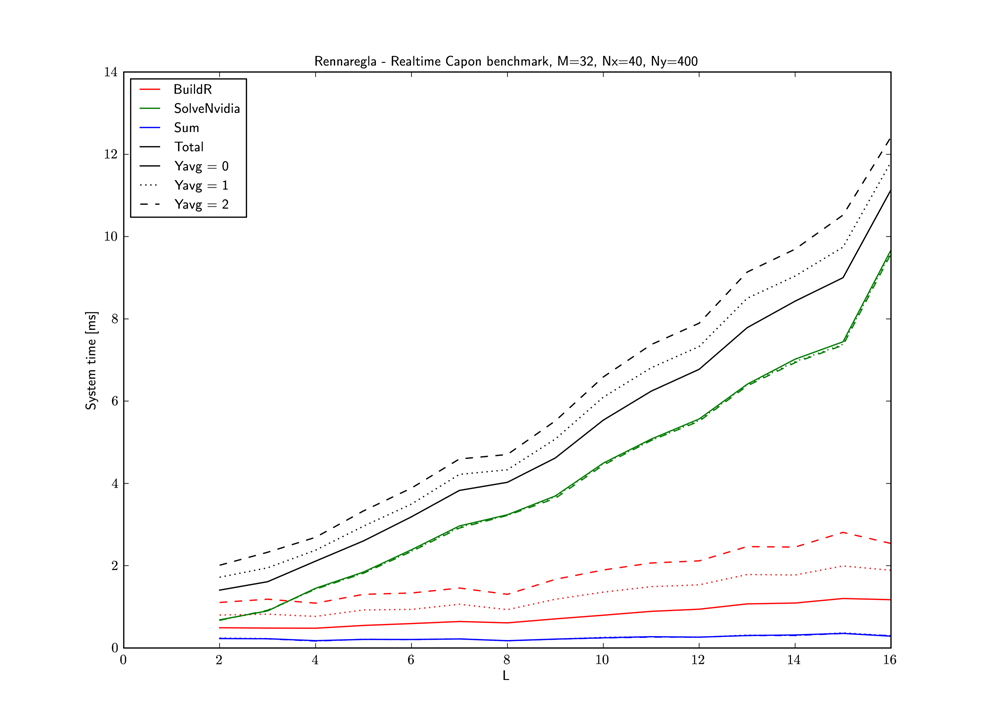
\includegraphics[width=3.9in]{gfx/benchmark_us_32_lr.png} \label{fig:benchUS32}}
\hfil
\subfloat[]{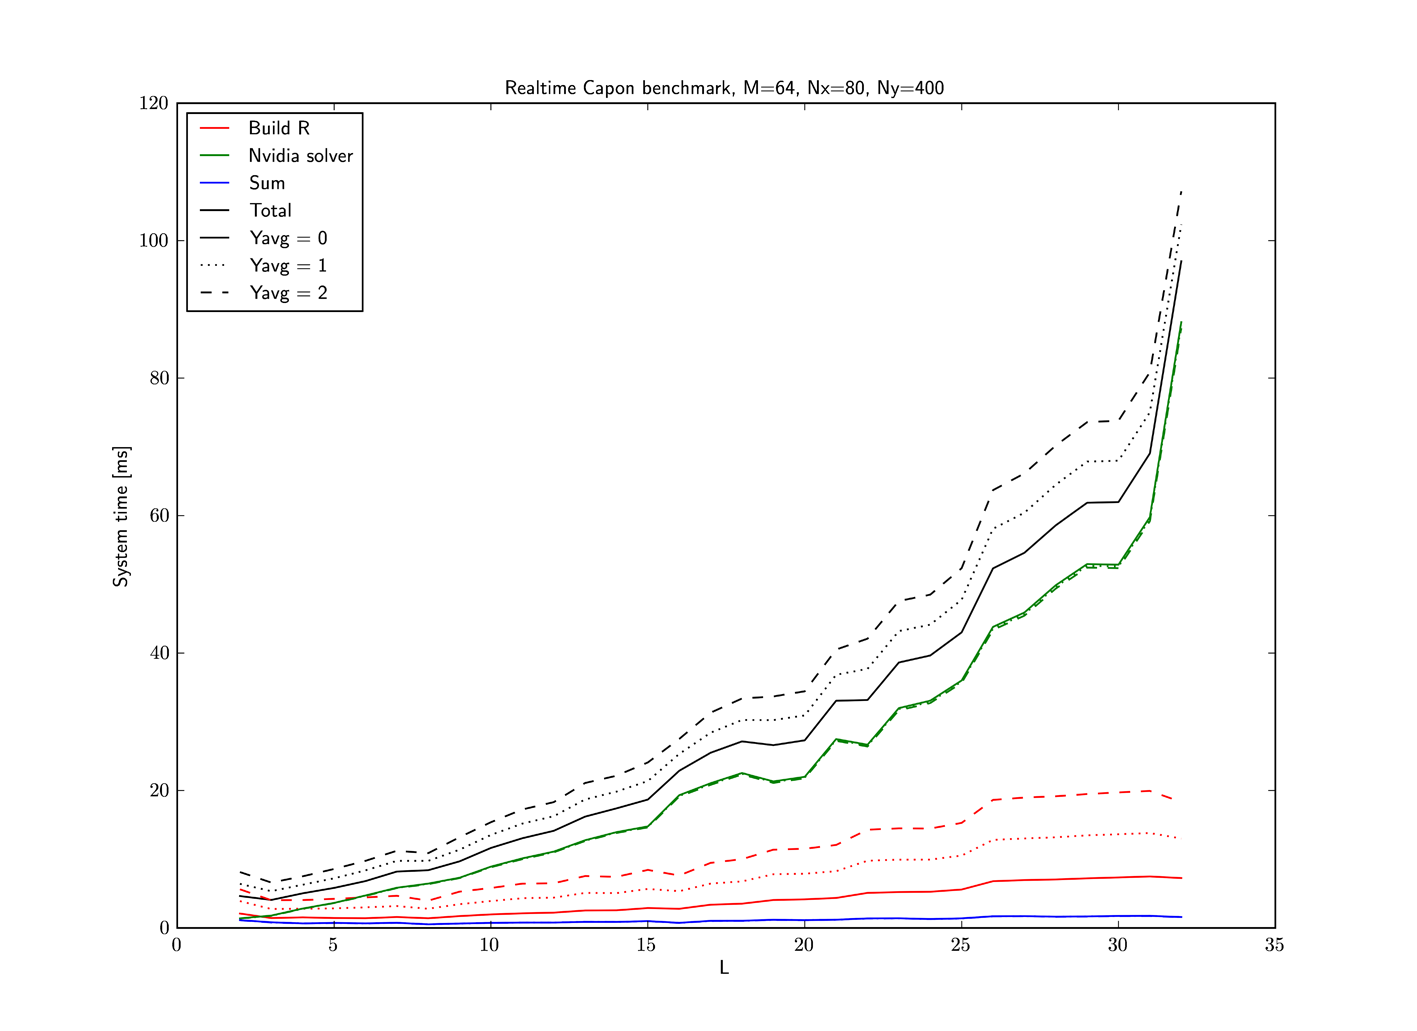
\includegraphics[width=3.9in]{gfx/benchmark_us_64_lr.png}%
\label{fig:benchUS64}}}
\caption{Benchmark of GPU Capon beamforming for a cardiac image covering a $70\degree$ sector. Execution time is plotted as a function of subarray length $L \in [1, M/2]$. The plot shows execution times for the three steps listed in Section \ref{sec:meth}: Calculation of covariance matrices in red, solver in green, and the final beamformer sum in blue. For each step, there is one line per choice of temporal averaging, $K \in [0, 1, 2]$. (a) A 32 element array. (b) A 64 element array.}
\label{fig:bench}
\end{figure*}

\section{Benchmarks and Videos}
Figure \ref{fig:bench} shows the results from benchmarking the implementation described in Section \ref{sec:meth} on a Nvidia Quadro 6000 graphics card (14 SMs, 1 TFlops single precision, 6 GB global memory, and 144 GB/s memory bandwidth). The problem sizes are calculated based on 32 and 64 element arrays with center frequency 2.5 MHz. By assuming a system bandwidth of 80\% we need a complex sampling frequency of 2 MHz. If we image down to a depth of 15 cm we get approximately 400 samples per range line. To correctly sample a $70\degree$ sector with 64 and 32 element arrays ($\lambda/2$ pitch) we need at least 80 and 40 beams respectively. The presented execution times do not include transfer of data from CPU-side to the GPU. What is included are all calculations, memory transfers from global to near-core GPU memory, and near core memory access. 

In the attached videos one will find a cardiac loop (add ref to video), and a simulated phantom (add ref to videos) processed with different types of settings given to the Capon beamformer. Cardiac data was acquired using a 64 element and 3.5 MHz phased array. Simulations were done using a 64 element 2.5 MHz phased array. 

\section{Discussion}
From Figure \ref{fig:benchUS64} we see that for $L = M/2 = 32$ and $K=1$, total execution time is 100 ms (10 fps). Taking into account that we use complex data, but less samples per image, this is similar to the performance reported by Chen et al. \cite{Chen2011}. For the 32 element array in Figure (\ref{fig:benchUS32}), execution time is reduced to 11.5 ms (87 fps) using the same settings ($L=M/2, K = 1$). Doubling this number can be interpreted as pre-beamforming a 64 element array down to 32. The frame rate for a 64 element array is then increased from 10 to 44 fps.

A major part of the total execution time comes from solving systems of linear equations. Further research should therefore focus on making this contribution smaller. This can be done either by implementing faster solvers, or reducing the sample covariance matrix size in a novel way (ref?). When doing such a reduction, including the pre-beamforming described above, one should investigate the loss of contrast and resolution compared with full Capon beamforming.

As for now, we have shown that the Capon beamformer can be implemented in a GPU framework. And if we as in \cite{Chen2011} define real-time as 10 fps, all execution times  in Figure (\ref{fig:bench}) are real time. If we on the other hand define real-time as the time it takes to acquire a given image. The image formed using a 32 and 64 element array has a real time requirement of 125 fps and 62.5 fps respectively. There is some distance to cover before that goal is reached for all values of $L \le M/2$. However we see, by the last definition, that real time is possible for $M=64, L < 16$, and for $M = 32, L < 13$. 

(Should comment on videos)

%Do we need more beams? 

% cite field II

% An example of a floating figure using the graphicx package.
% Note that \label must occur AFTER (or within) \caption.
% For figures, \caption should occur after the \includegraphics.
% Note that IEEEtran v1.7 and later has special internal code that
% is designed to preserve the operation of \label within \caption
% even when the captionsoff option is in effect. However, because
% of issues like this, it may be the safest practice to put all your
% \label just after \caption rather than within \caption{}.
%
% Reminder: the "draftcls" or "draftclsnofoot", not "draft", class
% option should be used if it is desired that the figures are to be
% displayed while in draft mode.
%
%\begin{figure}[!t]
%\centering
%\includegraphics[width=2.5in]{myfigure}
% where an .eps filename suffix will be assumed under latex, 
% and a .pdf suffix will be assumed for pdflatex; or what has been declared
% via \DeclareGraphicsExtensions.
%\caption{Simulation Results}
%\label{fig_sim}
%\end{figure}

% Note that IEEE typically puts floats only at the top, even when this
% results in a large percentage of a column being occupied by floats.


% An example of a double column floating figure using two subfigures.
% (The subfig.sty package must be loaded for this to work.)
% The subfigure \label commands are set within each subfloat command, the
% \label for the overall figure must come after \caption.
% \hfil must be used as a separator to get equal spacing.
% The subfigure.sty package works much the same way, except \subfigure is
% used instead of \subfloat.
%
%\begin{figure*}[!t]
%\centerline{\subfloat[Case I]\includegraphics[width=2.5in]{subfigcase1}%
%\label{fig_first_case}}
%\hfil
%\subfloat[Case II]{\includegraphics[width=2.5in]{subfigcase2}%
%\label{fig_second_case}}}
%\caption{Simulation results}
%\label{fig_sim}
%\end{figure*}
%
% Note that often IEEE papers with subfigures do not employ subfigure
% captions (using the optional argument to \subfloat), but instead will
% reference/describe all of them (a), (b), etc., within the main caption.


% An example of a floating table. Note that, for IEEE style tables, the 
% \caption command should come BEFORE the table. Table text will default to
% \footnotesize as IEEE normally uses this smaller font for tables.
% The \label must come after \caption as always.
%
%\begin{table}[!t]
%% increase table row spacing, adjust to taste
%\renewcommand{\arraystretch}{1.3}
% if using array.sty, it might be a good idea to tweak the value of
% \extrarowheight as needed to properly center the text within the cells
%\caption{An Example of a Table}
%\label{table_example}
%\centering
%% Some packages, such as MDW tools, offer better commands for making tables
%% than the plain LaTeX2e tabular which is used here.
%\begin{tabular}{|c||c|}
%\hline
%One & Two\\
%\hline
%Three & Four\\
%\hline
%\end{tabular}
%\end{table}


% Note that IEEE does not put floats in the very first column - or typically
% anywhere on the first page for that matter. Also, in-text middle ("here")
% positioning is not used. Most IEEE journals/conferences use top floats
% exclusively. Note that, LaTeX2e, unlike IEEE journals/conferences, places
% footnotes above bottom floats. This can be corrected via the \fnbelowfloat
% command of the stfloats package.



%\section{Conclusion}
%The conclusion goes here.




% conference papers do not normally have an appendix


% use section* for acknowledgement
\section*{Acknowledgment}
The authors would like to thank Tore Bj\aa{}stad at GE Vingmed Ultrasound for providing cardiac data, and Nvidia for their batched solver written in CUDA. 





% trigger a \newpage just before the given reference
% number - used to balance the columns on the last page
% adjust value as needed - may need to be readjusted if
% the document is modified later
%\IEEEtriggeratref{8}
% The "triggered" command can be changed if desired:
%\IEEEtriggercmd{\enlargethispage{-5in}}

% references section

% can use a bibliography generated by BibTeX as a .bbl file
% BibTeX documentation can be easily obtained at:
% http://www.ctan.org/tex-archive/biblio/bibtex/contrib/doc/
% The IEEEtran BibTeX style support page is at:
% http://www.michaelshell.org/tex/ieeetran/bibtex/
\bibliographystyle{IEEEtran}
% argument is your BibTeX string definitions and bibliography database(s)
\bibliography{mybib_conf}
%
% <OR> manually copy in the resultant .bbl file
% set second argument of \begin to the number of references
% (used to reserve space for the reference number labels box)
%\begin{thebibliography}{1}

%\bibitem{IEEEhowto:kopka}
%H.~Kopka and P.~W. Daly, \emph{A Guide to \LaTeX}, 3rd~ed.\hskip 1em plus
 % 0.5em minus 0.4em\relax Harlow, England: Addison-Wesley, 1999.

%\end{thebibliography}




% that's all folks
\end{document}


